\section{Quantity 3: Packing Density}

\intuitbox{More holes per unit area means more light through the array for a fixed
hole size --- this is the quantity being maximized once a design has
already passed the safety checks above. The tricky part is defining ``unit
area'' consistently: a regular lattice has an obvious repeating cell, but
an irregular pattern (a spiral, a jittered lattice) does not. Using
different area formulas for different families is exactly the bug that
made one family look artificially better than another earlier in this
project --- one consistent formula for every family fixes that.
}
\subsection{The Formula}
\begin{equation}
\text{Area} = \text{Hull}_{\text{area}} + \text{Hull}_{\text{perimeter}}\times R_h + \pi R_h^2
\end{equation}
\begin{equation}
\text{density} = \frac{N}{\text{Area}}
\end{equation}
This is the convex hull of the hole centers, expanded outward by one hole
radius (a Minkowski buffer) --- accounting for the fact that each hole
physically extends past its own center point, which the bare hull area
ignores.

\begin{figure}[h]
\centering
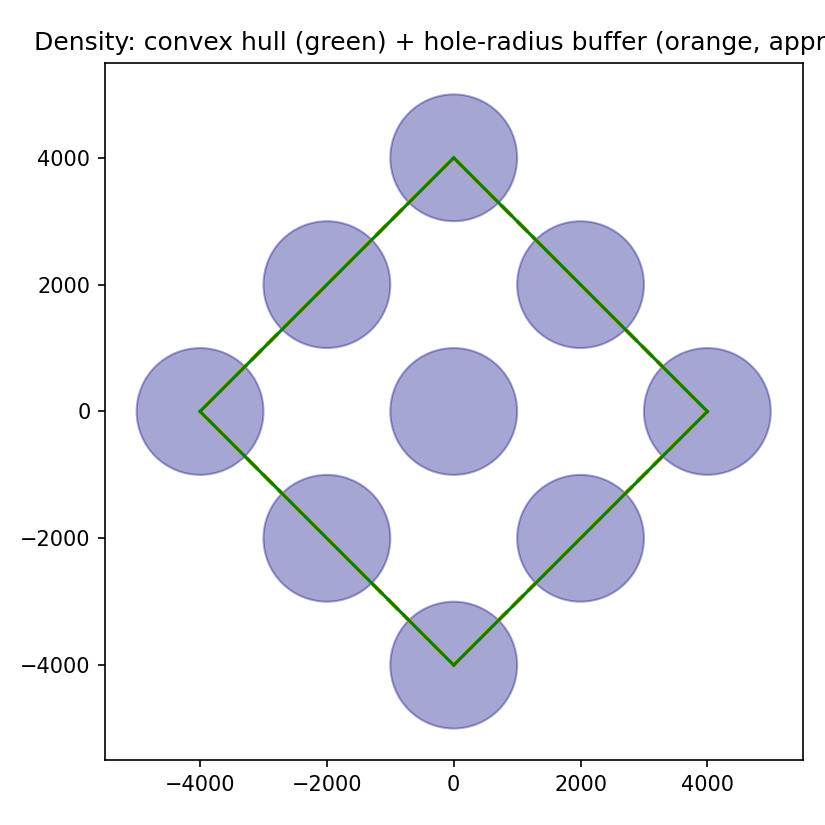
\includegraphics[width=0.55\textwidth]{verification_pdf_figs/fig_density.png}
\caption{Convex hull of the 9 hole centers (green) with an approximate
radius buffer (orange, dashed) for the worked example of Sec.~5.}
\end{figure}

\checkbox{List the hole coordinates for a small design (fewer than \raise0pt\hbox{$\sim$}15
holes is easiest by hand). Compute the convex hull area (the shoelace
formula works directly on the hull vertices). Add the hull perimeter times
$R_h$, plus $\pi R_h^2$. Divide $N$ by this total. Compare against the
pipeline's own reported density for that exact row --- they should match to
within rounding.
}
\newpage
